\chapter*{Dodatak: Prikaz aktivnosti grupe}
		\addcontentsline{toc}{chapter}{Dodatak: Prikaz aktivnosti grupe}
		
		\section*{Dnevnik sastajanja}
		
		
		
		\begin{packed_enum}
			\item  sastanak
			
			\item[] \begin{packed_item}
				\item Datum: 20.\ listopada 2023.
				\item Prisustvovali: svi
				\item Teme sastanka:
				\begin{packed_item}
					\item  odabir razvojnih alata i tehnologija
					\item  generalna podjela poslova
				\end{packed_item}
			\end{packed_item}
			
			\item  sastanak
			\item[] \begin{packed_item}
				\item Datum: 25.\ listopada 2023.
				\item Prisustvovali: svi
				\item Teme sastanka:
				\begin{packed_item}
					\item  detaljnija podjela poslova
					\item  rasprava oko funkcionalnih i nefunkcionalnih zahtjeva
				\end{packed_item}
			\end{packed_item}

			\item  sastanak
			\item[] \begin{packed_item}
				\item Datum: 26.\ listopada 2023.
				\item Prisustvovali: Filip Krilčić, Vilim Branica, Lovro Mužar
				\item Teme sastanka:
				\begin{packed_item}
					\item  organizacija baze podataka
					\item  dijagrami i implementacija baze podataka
				\end{packed_item}
			\end{packed_item}
			
			\item  sastanak
			\item[] \begin{packed_item}
				\item Datum: 27.\ listopada 2023.
				\item Prisustvovali: Filip Krilčić, Vilim Branica, Zvonimir Pipić, Nika Miličević, Marko Šelendić, Lovro Mužar
				\item Teme sastanka:
				\begin{packed_item}
					\item  završavanje prošlo podijeljenih poslova te provjera prethodno završenog posla
					\item  podijela novih poslova - OCR demo, dokumentacija (Sekvencijski dijagrami te opis projekta), opis baze i početna stranica, te određivanje roka za završetak istih
				\end{packed_item}
			\end{packed_item}
			
			\item  sastanak
			\item[] \begin{packed_item}
				\item Datum: 28.\ listopada 2023.
				\item Prisustvovali: Filip Krilčić, Vilim Branica i Zvonimir Pipić
				\item Teme sastanka:
				\begin{packed_item}
					\item  podjela poslova na backendu
				\end{packed_item}
			\end{packed_item}
			
			\item  sastanak
			\item[] \begin{packed_item}
				\item Datum: 4.\ studenoga 2023.
				\item Prisustvovali: Filip Krilčić, Vilim Branica, Zvonimir Pipić, Nika Miličević, Marko Šelendić, Tomislav Čupić
				\item Teme sastanka:
				\begin{packed_item}
					\item  analiza commitanih fileova
					\item  prezentacija izrađenih osnovnih funkcionalnosti backenda
				\end{packed_item}
			\end{packed_item}

			\item  sastanak
			\item[] \begin{packed_item}
				\item Datum: 12.\ prosinca 2023.
				\item Prisustvovali: svi
				\item Teme sastanka:
				\begin{packed_item}
					\item  podjela bodova 1. revizije
					\item  analiza riješenih zadataka
					\item  određivanje preostalih zadataka 
				\end{packed_item}
			\end{packed_item}

   			\item  sastanak
			\item[] \begin{packed_item}
				\item Datum: 16.\ prosinca 2023.
				\item Prisustvovali: Marko Šelendić, Tomislav Čupić, Zvonimir Pipić
				\item Teme sastanka:
				\begin{packed_item}
					\item  podjela poslova na frontendu
				\end{packed_item}
			\end{packed_item}

			\item  sastanak
			\item[] \begin{packed_item}
				\item Datum: 13.\ siječnja 2024.
				\item Prisustvovali: svi
				\item Teme sastanka:
				\begin{packed_item}
					\item  pregled svih napravljenih funkcionalnosti, provjera rada aplikacije i ispravljanje sitnih grešaka 
				\end{packed_item}
			\end{packed_item}

		\end{packed_enum}
		
		\eject{}
		\section*{Tablica aktivnosti}
		
			\textbf{\textit{Kontinuirano osvježavanje}}\\
			
			 \textit{Napomena: Doprinose u aktivnostima treba navesti u satima po članovima grupe po aktivnosti.}

			\begin{longtblr}[
					label=none,
				]{
					vlines,hlines,
					width = \textwidth,
					colspec={X[7, l]X[1, c]X[1, c]X[1, c]X[1, c]X[1, c]X[1, c]X[1, c]}, 
					vline{1} = {1}{text=\clap{}},
					hline{1} = {1}{text=\clap{}},
					rowhead = 1,
				} 
			
				\SetCell[c=1]{c}{} & \SetCell[c=1]{c}{\rotatebox{90}{\textbf{Vilim Branica}}} & \SetCell[c=1]{c}{\rotatebox{90}{\textbf{Tomislav Čupić}}} &	\SetCell[c=1]{c}{\rotatebox{90}{\textbf{Filip Krilčić}}} & \SetCell[c=1]{c}{\rotatebox{90}{\textbf{Nika Miličević}}} &	\SetCell[c=1]{c}{\rotatebox{90}{\textbf{Lovro Mužar}}} & \SetCell[c=1]{c}{\rotatebox{90}{\textbf{Zvonimir Pipić}}} &	\SetCell[c=1]{c}{\rotatebox{90}{\textbf{Marko Šelendić}}} \\  
				Upravljanje projektom 		& 21 &  &  &  &  &  &  \\ 
				Opis projektnog zadatka 	&  & 2 &  &  &  &  &  \\ 
				
				Funkcionalni zahtjevi       & 1 & 3 &  &  & 1 & 1 & 3  \\ 
				Opis pojedinih obrazaca 	&  &  &  &  &  &  & 3  \\ 
				Dijagram obrazaca 			&  &  &  & 6 &  &  &  \\ 
				Sekvencijski dijagrami 		&  &  &  & 7 &  &  &  \\ 
				Opis ostalih zahtjeva 		&  & 1 &  &  &  &  &  \\ 

				Arhitektura i dizajn sustava	 &  & 1 &  &  &  & 4 &  \\ 
				Baza podataka				&  &  & 5 &  &  &  &  \\ 
				Dijagram razreda 			&  &  &  & 12 &  &  &  \\ 
				Dijagram stanja				&  &  &  &  &  &  &  \\ 
				Dijagram aktivnosti 		&  &  &  &  &  &  &  \\ 
				Dijagram komponenti			&  &  &  &  &  &  &  \\ 
				Korištene tehnologije i alati 		&  &  & 1 &  &  &  &  \\ 
				Ispitivanje programskog rješenja 	&  &  &  &  &  &  &  \\ 
				Dijagram razmještaja			&  &  &  &  &  &  &  \\ 
				Upute za puštanje u pogon 		&  &  &  &  & 2 &  &  \\  
				Dnevnik sastajanja 			&  & 2 & 1 &  &  &  & 1  \\ 
				Zaključak i budući rad 		&  &  & 1 &  &  &  &  \\  
				Popis literature 			&  &  & 0.5 &  &  &  &  \\  
				&  &  &  &  &  &  &  \\ \hline 
				\textit{Frontend} 	&  & 25 &  &  &  &  & 30 \\  
				\textit{Backend (views i slično)} 	& 25 &  & 25 &  &  &  &  \\ 
    			\textit{Povezivanje frontenda i backenda} 	& 20 & 5 &  &  &  &  & 20 \\  
				\textit{Izrada opisa baze} 	& 10 &  & 10 &  & 4 & 2 &  \\ 
				\textit{Implementacije baze} 	& 8 &  & 7 &  &  &  &  \\ 
				\textit{Povezivanje na vanjski API za upload slike} &  &  & 5 &  &  & 10 &  \\
				\textit{Implementacija OCR-a} 	&  &  &  &  & 55 &  &  \\
				\textit{Deployment} 	& 10 &  &  &  & 45 &  & 10 \\
			\end{longtblr}
					
					
		\eject
		\section*{Dijagrami pregleda promjena}
		
		\begin{figure}[H]
			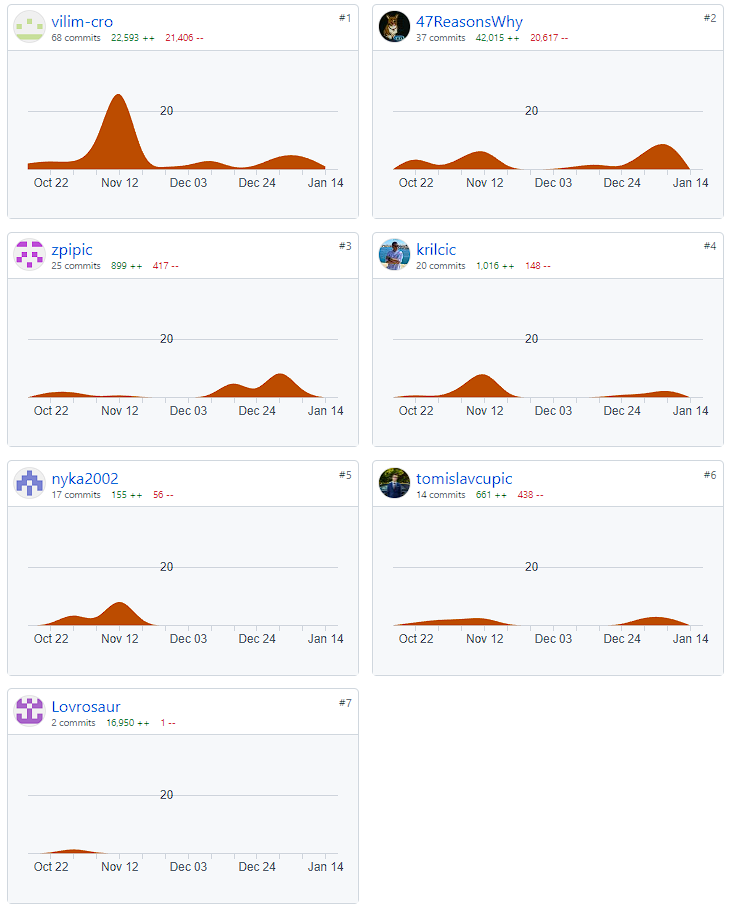
\includegraphics[width=\textwidth]{slike/git_aktivnost.png}
			\caption{Prikaz aktivnosti na repozitoriju}
			\label{fig:aktivnost}
		\end{figure}
		\eject 
	
